\tikzset{   cirwhite/.style={draw=gray,circle,fill=white,minimum size=20pt,inner sep=2pt,line width=0.2mm},
            cirred/.style={draw=gray,circle,fill=red,minimum size=20pt,inner sep=2pt,line width=0.2mm},
}

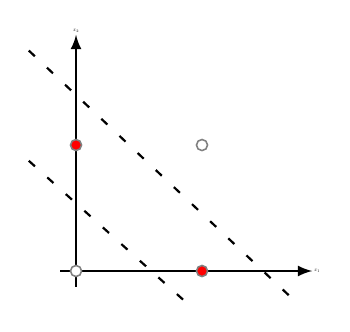
\begin{tikzpicture}[thick,scale=0.2, every node/.style={scale=0.2}]
    \draw[|->, -latex, draw] (-1,0) -- (15,0); %draw axis
    \draw[|->, -latex, draw] (0,-1) -- (0,15);

    \node[anchor=west] at (15,0) {$x_1$};  % draw axis labels
    \node[anchor=south] at (0,15) {$x_2$};

    \draw[loosely dashed] (-3,7) -- (7,-2);    % draw diagonal lines
    \draw[loosely dashed] (-3,14) -- (14,-2);

    \node[cirwhite] at (0,0) {}; % circles
    \node[cirred] at (0,8) {};
    \node[cirred] at (8,0) {};
    \node[cirwhite] at (8,8) {};
\end{tikzpicture}